\subsection{Test-case search problem}
\label{sec:problem}

\begin{figure}
\centering
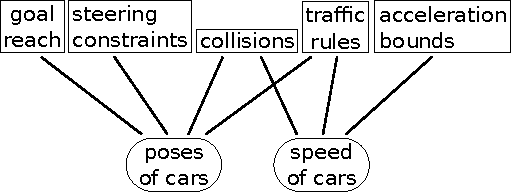
\includegraphics[width=70mm]{figures/chapter4/problem.pdf}%
\caption{Test-case CSP problem.}
\label{fig:problem}%
\end{figure}

%---search variables and parameters
The \emph{search variables} are the behaviors of the new non-egos, a \emph{complexity certificate}, and a \emph{solvability certificate}.
%
The \emph{complexity certificate} is an ego behavior that solves the old test-case, but fails the new test-case.
%
The \emph{solvability certificate} is an ego behavior that solves the new test-case.
%
The set of new non-egos and their routes through the intersection are given as parameters rather than as search variables.%
\footnote{The reason we did not extend our algorithm to automatically select values for these parameters is that it is not clear how to do significantly better than a brute-force approach.
%
Furthermore, a manual parameter assignment gives more control over the search.}
%
As discussed in the previous section, we do not change the behaviors of the old non-egos so they are fixed parameters.
%
The rest of the parameters, such as the scenery and traffic rules, are given by the old test-case.


%---constraints
There are three types of constraints imposed by the pass-fail criteria, to generate a more-complex and solvable test-case.
%
First is collision avoidance, which regards the shape of each car, and its location and orientation at each time relative to other cars.
%
The locations and orientations are themselves constrained by physics, such as limited forces available to accelerate or brake, and bounded range for steering angles.
%
Second is goal-reach, which regards overlap of a trajectory with a region in the scenery.
%
This in turn is constrained by physics of car motion, and also the scenery.
%
Third is traffic rules, which regards the lane events, stop events, etc.
%
This depends on the logic of traffic rules, geometry of lanes, location and orientation of the cars at each time, also each car's shape.
%
The space of possible complexity and solvability certificates depends on the choice of new non-ego behaviors.
%
Therefore, the search for the new non-egos has to be done simultaneously as the search for the certificates.


%---proposed strategy
Our proposed approach is to decompose the CSP problem into three subproblems, where each subproblem is suitable to a specialized technique.
%
In particular, we use simulation and closed-loop control to find a sequence of poses that satisfies the steering constraints and goal-reach.
%
We use ASP to find possible orderings of events that satisfy the required traffic rules violations or compliance.
%
Finally, we use SMT to find timing of poses that satisfy the analytical constraints on the longitudinal motion e.g. smoothness of speed, bounded longitudinal acceleration, negligible speed at stop events, etc.
%
Our decomposition of the problem is shown in Figure~\ref{fig:problem}.
%
The first subproblem finds the poses of cars, while the second and third subproblems find the speed of cars.


%---constraints on new non-egos
The new non-egos should not collide with the old non-egos since a collision may alter an old non-ego's trajectory which violates our guarantee of comparability of test-case complexities.


%---constraints on complexity certificate
The complexity certificate is an ego behavior that passes the old test-case, but fails the new test-case.
%
The constraints that guarantee such a behavior are as follows.
%
The behavior should avoid colliding with the old non-egos, respect traffic signs and the right-of-way of old non-egos, and reach ego's goal, to pass the old test-case.
%
The behavior should avoid colliding with the new non-egos, so that it is a physically valid behavior in the old test-case where the collision forces of the new non-egos are absent.
%
Since the behavior respects traffic signs and does not collide with the new non-egos, the only way for it to fail the new test-case is to violate the right-of-way of at least one of the new non-egos.


%---solvability certificate
The solvability certificate is an ego behavior that passes the new test-case.
%
That is, the behavior does not collide with the old or new non-egos, respects traffic signs and the right-of-way of both the old and new non-egos, and reaches ego's goal.






